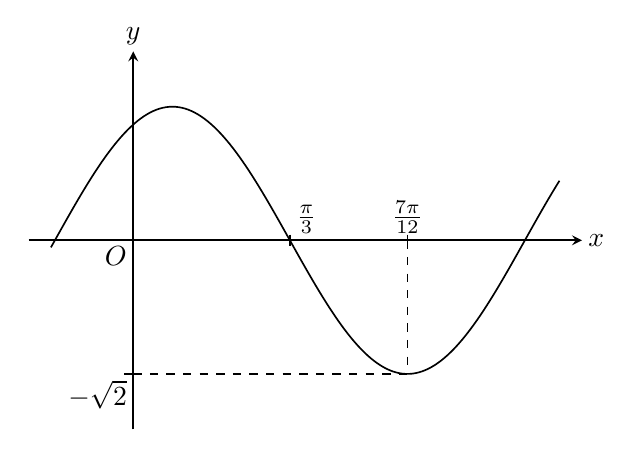
\begin{tikzpicture}[x=1.9cm,y=1.2cm,line width=.6pt,>=stealth]
\draw[->] (-0.7,0)--(3.0,0) node[right,inner sep=0pt,xshift=2pt] {$x$};
\draw[->] (0,-2.0)--(0,2.0) node[above,inner sep=0pt,yshift=2pt] {$y$};
\node[below left,inner sep=0pt,xshift=-2pt,yshift=-2pt] at (0,0) {$O$};
\draw (1.0472,0.06)--(1.0472,-0.06);
\node[above right,inner sep=0pt,xshift=2pt,yshift=2pt] at (1.0472,0) {$\frac{\pi}{3}$};
\draw (1.8326,0.06)--(1.8326,-0.06);
\node[above,inner sep=0pt,yshift=2pt] at (1.8326,0) {$\frac{7\pi}{12}$};
\draw (-0.06,-1.4142)--(0.06,-1.4142);
\node[below left,inner sep=0pt,xshift=-2pt,yshift=-2pt] at (0,-1.4142) {$-\sqrt{2}$};
\draw[domain=-0.55:2.85,samples=160] plot (\x,{sqrt(2)*sin(deg(2*\x+pi/3))});
\draw[dashed] (1.8326,0)--(1.8326,-1.4142);
\draw[dashed] (0,-1.4142)--(1.8326,-1.4142);
\end{tikzpicture}
